\documentclass[discrete.tex]{subfiles}

\begin{document}

\section{Деревья. Теорема о шести эквивалентных определениях дерева}

\begin{theorem}
    \begin{enumerate}
        \item Cвязный граф без циклов
        \item Связный граф, в котором дуг на 1 меньше, чем вершин
        \item Граф без циклов, в котором дуг на 1 меньше, чем вершин
        \item Минимальный связный граф, т.е граф, который при удалении любого ребра перестает быть связным
        \item Максимальный граф без циклов
        \item Граф, в котором две любые вершины соединены цепью и притом только одной
    \end{enumerate}
\end{theorem}

\begin{Proof} \
  \begin{figure}[H]
          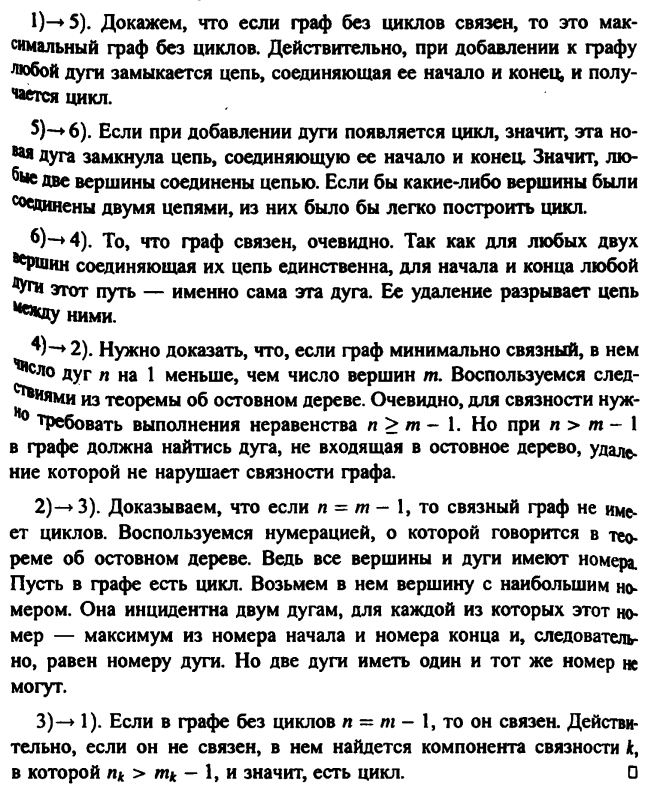
\includegraphics[width=10cm]{pics/42_1}
          \centering
  \end{figure}
\end{Proof}

\end{document}
